\chapter{Projekt aplikacji}
	Podczas projektowania aplikacji, ustalono jej wymaganie funkcjonalne oraz niefunkcjonalne. Opracowano strukturę projektu, która zakłada podział programu na trzy mniejsze części. Zamieszczono diagramy UML przedstawiające publiczne interfejsy programistyczne tych modułów.
	
	\section{Wymagania funkcjonalne}
	Założono, że aplikacja będzie posiadać graficzny interfejs użytkownika umożliwiający podgląd i modyfikacje stanów wewnętrznych procesora, takich jak rejestry, pamięć i~flagi. Możliwe będzie wykonanie dwóch trybów emulacji, ciągły oraz krokowy. 
	W widocznym miejscu zostaną umiejscowione informacje o liczbie wykonanych cykli maszynowych i zegara.
	Aplikacja pozwoli na zgłaszanie przerwań maskowalnych i niemaskowalnych oraz wprowadzenia wartości szyny danych, jaką ustaliłoby urządzenie wywołujące przerwanie podczas zgłoszenia. 
	Użytkownikowi zostanie udostępniona możliwość wprowadzenia kodu asemblera do aplikacji, skompilowanie go i wczytanie do pamięci. Podczas emulacji zostanie wyświetlona nazwa poprzedniej i następnej wykonanej instrukcji procesora.

	\section{Wymagania niefunkcjonalne}
	Podstawowym założeniem, jest możliwość uruchomienia aplikacji na jak największej liczbie platform. Jako minimum zdecydowano się na systemy operacyjne \emph{MS Windows}, \emph{Ubuntu} i \emph{Mac OS}. Instrukcje procesora powinny być wykonywane bezbłędnie, zgodnie z dokumentacją techniczną procesora. Projekt powinien mieć interfejs programistyczny umożliwiający podłączenia go z innymi aplikacjami, np. emulatorami urządzeń, które do swojej pracy wykorzystują Ziloga Z80.
	
	\section{Struktura aplikacji}
	Aplikację podzielono na trzy moduły: \emph{Xbit}, \emph{Z80emu{\dywiz}core} oraz \emph{Z80emu{\dywiz}gui}, z~których każdy jest osobnym modułem. Zależności między nimi pokazuje diagram \ref{img:strutkuraAplikacji}. Moduł \emph{XBit} do swojego działania nie wymaga innych modułów. \emph{Z80emu{\dywiz}core} potrzebuje modułu \emph{XBit} do poprawnego działania i jest on jego częścią, natomiast \emph{X80emu{\dywiz}gui} zawiera w sobie \emph{Z80emu{\dywiz}core}, a co za tym idzie także \emph{Xbit}.
    
    \begin{figure}[h]
		\centering
		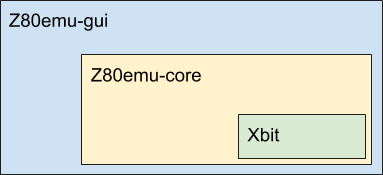
\includegraphics[width=0.6\textwidth]{strukturaAlikacji.png}
		\caption{Zależności pomiędzy modułami aplikacji}
		\label{img:strutkuraAplikacji}
	\end{figure}
    
	\section{Biblioteka XBit}
	Java jest językiem programowania wysokiego poziomu, kompilowanym do kodu bajtowego. Z tego powodu nie jest on zazwyczaj stosowany w emulacji, gdyż kod emulatora musi być uruchamiany w maszynie wirtualnej, co nie jest wydajnym rozwiązaniem.

	Innym poważnym problemem języka Java jest brak typów prostych pozwalających przechowywać wyłącznie liczby dodatnie. Problem rozwiązuje biblioteka XBit. Zawiera ona klasy, które umożliwiają przechowywanie wartości jedno i dwu bajtowych. Mogą one zostać zinterpretowane jako liczby zapisane w kodzie dopełnień do dwóch (liczby dodatnie i ujemne), lub naturalnym kodzie binarnym (tylko liczby dodatnie). \newline
	Przykładowo, liczba binarna 1110 odczytana w naturalnym kodzie binarnym (NKB), to 15 (w zapisie decymalnym), natomiast w kodzie dopełnień do dwóch (U2) to -2. XBit pozwala na obydwie interpretacje za pomocą odpowiednich metod, zwracając wynik jako typ prymitywny \emph{int}. 
	
	Nie jest to idealne rozwiązanie. Typ \emph{int} przechowuje cztero{\dywiz}bajtowe liczby z zakresu od -2 147 483 648 do 2 147 483 647, więc większość bajtów zostaje niewykorzystana. Nadmiarowość jest w tym przypadku wymagana, ponieważ zakres liczb w notacji NKB i~w~U2 jest inny.
	
	Przykładowo, w przypadku gdy za pomocą XBit stworzono reprezentację liczby ośmio bitowej: \newline1111 0000 (w kodzie jest to NKB=240, U2=-16) to wywołując metodę interpretującą ją jako liczba bez znaku (czyli w notacji NKB), zostanie zwrócona zmienna o typie prymitywnym \emph{int}, o wartości 240,  binarne \newline 00000000 00000000 00000000 11110000. \newline
	Natomiast jeśli wykonamy metodę interpretującą ją jako liczba ze znakiem (czyli w notacji U2) zostanie zwrócona wartość -16, binarnie \newline 11111111 11111111 11111111 11110000.\newline
    
    Bibliotekę zaprojektowano w taki sposób, aby była jak najbardziej uniwersalna, i można ją było wykorzystać do budowy emulatora Zilog-a Z80, ale także innych procesorów. 

	\subsection{Możliwości biblioteki XBit}
	Założono, że biblioteka \emph{XBit} będzie spełniała następujące wymagania:
	\begin{itemize}  
		\item reprezentacja liczb 8 i 16 bitowych,
		\item interpretacja liczb w naturalnym kodzie binarnym lub dopełnieniu do dwóch,
		\item operacje na pojedynczych bitach (możliwość zmiany, odczytu bitu na danej pozycji),
		\item opcja odczytania grupy bitów (odczytanie kilku bitów z~określeniem pozycji pierwszego i ostatniego bitu),
		\item interpretacja liczb 16 bitowych w formacie \emph{big endian} lub \emph{little endian},
		\item operacje arytmetyczne (dodawanie, odejmowanie),
		\item operacje bitowe na liczbach (negacja, alternatywa, koniunkcja, przesunięcia bitowe),
		\item uwzględnienie przy operacjach arytmetycznych przepełnienia oraz przeniesienia.
	\end{itemize} 
	
	\subsection{Założenia projektowe XBit}
	Przed przystąpieniem do implementacji rozwiązania, zaprojektowano publiczny interfejs biblioteki w języku UML, zaprezentowany na diagramie \ref{img:xbitUml}. Ustalono także założenia projektowe, które zaprezentowano poniżej. 
	
	\begin{figure}[h]
		\centering
		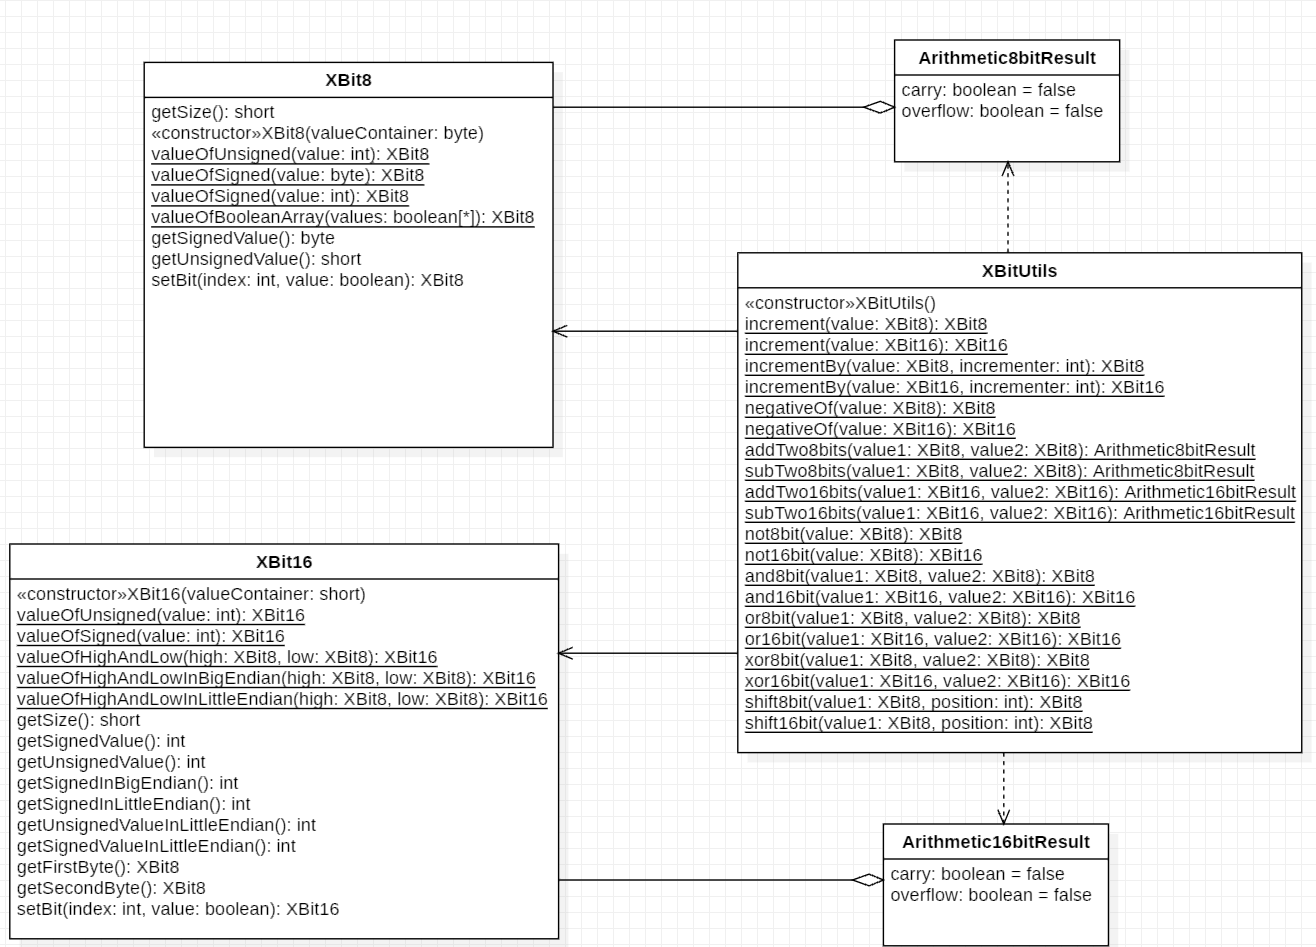
\includegraphics[width=1\textwidth]{xbitUml}
		\caption{Hierarchia klas biblioteki XBit}
		\label{img:xbitUml}
	\end{figure}
	
	\subsubsection{Klasy XBit8 i XBit16}
	Klasy \emph{XBit8} oraz \emph{XBit16} służą do reprezentowania liczb 8 i 16 bitowych. Postanowiono, że zmiana stanu wewnętrznego ich obiektów, czyli wartości w~nich przechowywanych będzie niemożliwa (są to obiekty niezmienne, z ang. \emph{immutable}), tak jak w~przypadku obiektowych reprezentacji typów prostych w języku Java (\emph{Short}, \emph{Long}, \emph{Integer} itp).  Konsekwencją tej decyzji jest to, że metody które powinny zmienić stan obiektu, klonują istniejący obiekt a następnie modyfikują odpowiednio stan jego kopii. Przykładem takiej metody jest \emph{setBit(index: int, value: boolean)} występująca w~obu klasach. Podprogram ten nie zmienia bitu obiektu na rzecz którego został wykonany, a jedynie zwraca kopie obiektu, ze zmodyfikowanym odpowiednim bitem. 
	
	Zalety zastosowania obiektów niezmiennych:
	\begin{itemize} 
		\item prosta implementacja oraz łatwe debugowanie kodu,
		\item \emph{Garbage Collector} jest przystosowany do pracy z tego typu obiektami,
		\item łatwość zapisywania obiektów do pliku lub pamięci podręcznej (z ang. \emph{cache}),
		\item bezpieczne używanie obiektów niezmiennych w programach wielowątkowych, co ułatwia emulacje procesorów wielopotokowych; jeden wątek w takim przypadku mógłby być odpowiedzialny za jeden stopień potoku, np osobny wątek odbierałby instrukcje z pamięci, inny by je dekodował, kolejny wykonywał i tak dalej,
		\item Możliwość użycia obiektu jako klucza, np. w \emph{HashMap}. 
	\end{itemize}

	Wadą zastosowania obiektów niezmiennych jest zwiększone użycie pamięci, co mimo wszystko nie powinno być przeszkodą dla współczesnych komputerów. Ze względu na przewagę zalet w stosunku do jednej wady postanowiono użyć tego typu obiektów niezmiennych w bibliotece.
	
	\subsubsection{Klasy XBitUtils, Arithmetic8bitResult, Arithmetic16bitResult}
	Klasa \emph{XBitUtils} jest odpowiedzialna za wszystkie operacje arytmetyczne oraz bitowe. Większość z jej metod zwraca obiekty klas \emph{XBit8} lub \emph{XBit16}. Wyjątkami są metody wykonujące dodawanie lub odejmowanie, które oprócz zwrócenia wyniku operacji, informują o wystąpieniu przeniesienia lub przepełnienia. Ponieważ język Java, jako wynik metody może zwrócić tylko jeden obiekt, postanowiono zaprojektować klasy \emph{Arithmetic8bitResult} oraz \emph{Arithmetic16bitResult} które grupują te trzy informacje w jedną klasę, której instancja zostanie zwrócona po wykonaniu operacji arytmetycznej. Klasy te zawierają następujące pola:
	\begin{itemize}
		\item obiekt klasy \emph{XBit8} lub \emph{XBit16} będący rezultatem operacji,
		\item dwie zmienne typu \emph{boolean} informujące o wystąpieniu przeniesienia i przepełnienia.
	\end{itemize}
	
	\section{Z80emu{\dywiz}core} \label{project:z80EmuCore}
	\emph{Z80emu{\dywiz}core} to moduł mający za zadanie wykonywać emulację oraz udostępniać zestaw metod umożliwiający manipulacje tym procesem. Za cel obrano stworzenie takiego interfejsu, który pozwalałby na użycie \emph{Z80emu{\dywiz}core} w innych projektach, które emulują urządzenia zbudowane z~użyciem Ziloga Z80. Jako przykład można podać emulator przenośnej konsoli \emph{Game Boy} firmy \emph{Nintendo} z 1989 roku, której procesorem jest Zilog~Z80. 

	Wymagania projektowe względem modułu są następujące:
	\begin{itemize}  
		\item możliwość wykonania wszystkich 158 rozkazów procesora,
		\item istnienie zestawu metod umożliwiających zmianę stanów rejestrów,
		\item emulacja zewnętrznej pamięci,
		\item możliwość podłączenia emulowanych urządzeń wejścia/wyjścia,
		\item umożliwienie zgłaszania przerwań maskowanych i~niemaskowanych. (Z80 posiada dwa rodzaje przerwań).
	\end{itemize}
	
	\subsection{Publiczny interfejs modułu Z80emu{\dywiz}core}
	Publiczny zestaw metod służący do zarządzania procesem emulacji, jak i urządzeniem, pokazano na diagramie \ref{img:z80emuCoreUml}.
	
	Klasa Z80 zawiera zestaw metod sterujących emulacją, oraz wartościami liczników i~mniejszych rejestrów procesora. Najważniejsze z~nich to:
	\begin{itemize}  
		\item \emph{Z80(memory: Memory, ioDevice: IoDevice)} - konstruktor, przyjmujący dwa parametry wymagane do poprawnego działania. Parametry ,,memory" oraz ,,ioDevice" to obiekty reprezentujące moduł pamięci oraz urządzenie wejścia/wyjścia podłączone do procesora. Użytkownik używający modułu \emph{Z80emu{\dywiz}core} powinien samemu zaimplementować ich działanie, w~zależności od zastosowania, dla którego chce emulować urządzenie. 
		
		\item \emph{runOneInstruction()} - metoda wykonująca pojedynczą instrukcję procesora.
		
		\item \emph{makeInterupt(addressBus: XBit8), makeNonMaskableInterupt(addressBus: XBit8)} - metody powinny zostać wykonane między kolejnymi wywołaniami \emph{runOneInstruction()}. Ich zadaniem jest zgłaszanie przerwań. Parametr \emph{addressBus} to wartość jaka zostałaby ustalona na magistrali danych podczas przerwania, gdyby zostało ono wykonane w prawdziwym urządzeniu.
	\end{itemize}
	
	Procesor Zilog Z80 posiada dwa zestawy rejestrów ogólnego przeznaczenia (do nich należąc rejestry A,B,C,D,E,H,L,F oraz ich 16bitowe odpowiedniki). Takie rozwiązanie jest dogodne, w przypadku gdy procesor często wykonuje obsługę przerwań. W klasycznym podejściu, w~ramach obsługi przerwania zestaw rejestrów ogólnego przeznaczenia zapisywany jest na stosie, co jest czasochłonną operacją. Projektanci Ziloga Z80 postanowili stworzyć drugi alternatywny zestaw rejestrów ogólnego przeznaczenia, który jest używany podczas obsługi przerwania. W takim przypadku nie jest wymagane odłożenie wartości rejestrów na stos.
	
	W projekcie reprezentacją zestawu rejestrów ogólnego przeznaczenia jest klasa \emph{DuplicableRegisterSet}. Jej dwie instancje (jedna jako główny zestaw rejestrów, druga alternatywny) przechowuje klasa \emph{RegisterBank}, która posiada metody \emph{switchRegisterSet()}, \emph{switchRegisterSetToA()} i \emph{switchRegisterSetToB()} pozwalające na przełączanie głównego zestawu rejestrów. Metody typu \emph{getA()}, \emph{setA(value: XBit8)} to aliasy wykonujące te operacje na aktualnie aktywnym zestawie. 
	
	\begin{figure}[h]
		\centering
		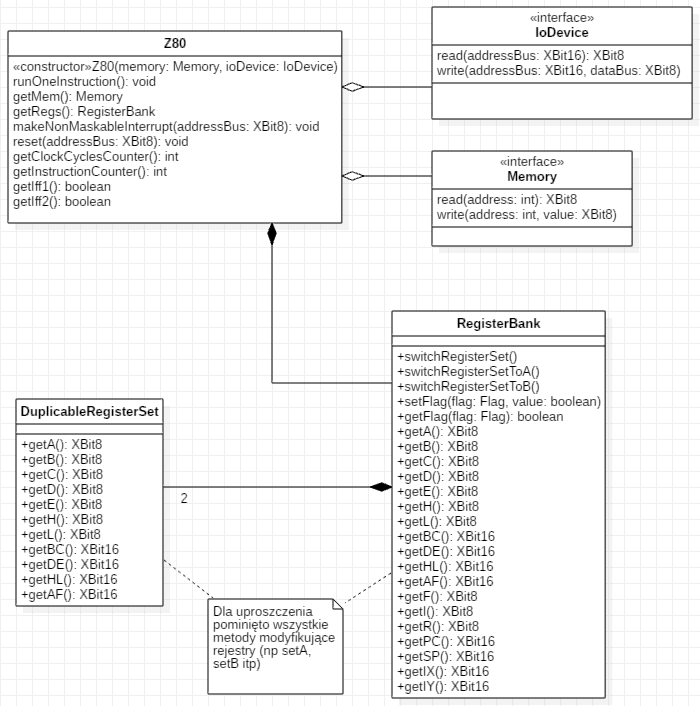
\includegraphics[width=0.9\textwidth]{z80emuCoreUml}
		\caption{Diagram hierarchii klas dla modułu z80emu{\dywiz}core}
		\label{img:z80emuCoreUml}
	\end{figure}
	
	\subsection{Łączenie z innymi projektami}
		
	Postanowiono nie uruchamiać procesu emulacji w pętli głównej tak jak w klasycznym podejściu pokazanym w kodzie \ref{listing:interpreter}. Zamiast tego udostępniono jedną metodę \emph{runOneInstruction()} która wykonuje jeden rozkaz procesora.
	
	Metody sterujące procesem emulacji (np. wywołanie przerwania, edycja rejestrów) powinny zostać wywoływane między kolejnymi wywołaniami \emph{runOneInstruction()}. Główna pętla emulacji powinna zostać zaimplementowania w module nadrzędnym, używającym \emph{z80emu{\dywiz}core}. Pozwala to na większą elastyczność modułu w łączeniu go z innymi projektami.
	
	Inną ważną decyzją projektową pozwalającą na zwiększenie elastyczności projektu, było zaprojektowanie interfejsów \emph{IoDevice} oraz \emph{Memory} i decyzja o zaimplementowaniu jedynie prostych reprezentacji klas implementujących te interfejsy.
	Aby uzasadnić powód wprowadzenia tego rozwiązania na rysunku \ref{img:z80minimalnySystemKomputerowy} przedstawiono minimalny system komputerowy oparty na procesorze Z80.
	Widać na nim, że pamięć programu (na rysunku jest to 8kb ROM) oraz podłączone urządzenie wejścia/wyjścia (na rysunku \emph{Z80-PIO}, który jest programowalnym układem wejścia/wyjścia) są osobnymi urządzeniami i mogą one być różne w zależności od systemu komputerowego. Interfejsy \emph{IoDevice} oraz \emph{Memory} pozwalają na implementację zachowania takich urządzeń, jakie są wymagane dla docelowego projektu. 
	
	
	\begin{figure}[h]
		\centering
		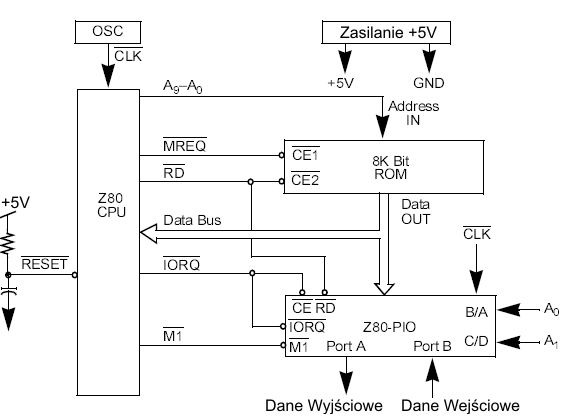
\includegraphics[width=0.6\textwidth]{z80minimalnySystemKomputerowy}
		\caption{Minimalny System Komputerowy Z80}
		\label{img:z80minimalnySystemKomputerowy}
	\end{figure}
		
	\section{Z80emu{\dywiz}gui}
	\emph{Z80emu{\dywiz}gui} to moduł realizujący interfejs użytkownika. Został on napisany z pomocą biblioteki \emph{JavaFX}. Projekt interfejsu obejmował stworzenie makiety w języku FXML zaprezentowanej na grafice \ref{img:z80Gui}. Większość interfejsów emulatorów posiada GUI złożone z wielu okien, które można dowolnie zamykać i otwierać, a każde z nich zawiera osobny moduł. Dla przykładu, w \emph{Z80 simulator IDE}, edytor pamięci, asembler lub manipulacja urządzeniami wejścia wyjścia zawarte są w osobnych oknach. 
	W projekcie \emph{Z80emu{\dywiz}gui} postanowiono stworzyć interfejs zawierający wszystkie funkcje w jednym oknie. 
	
	\begin{figure}[h]
		\centering
		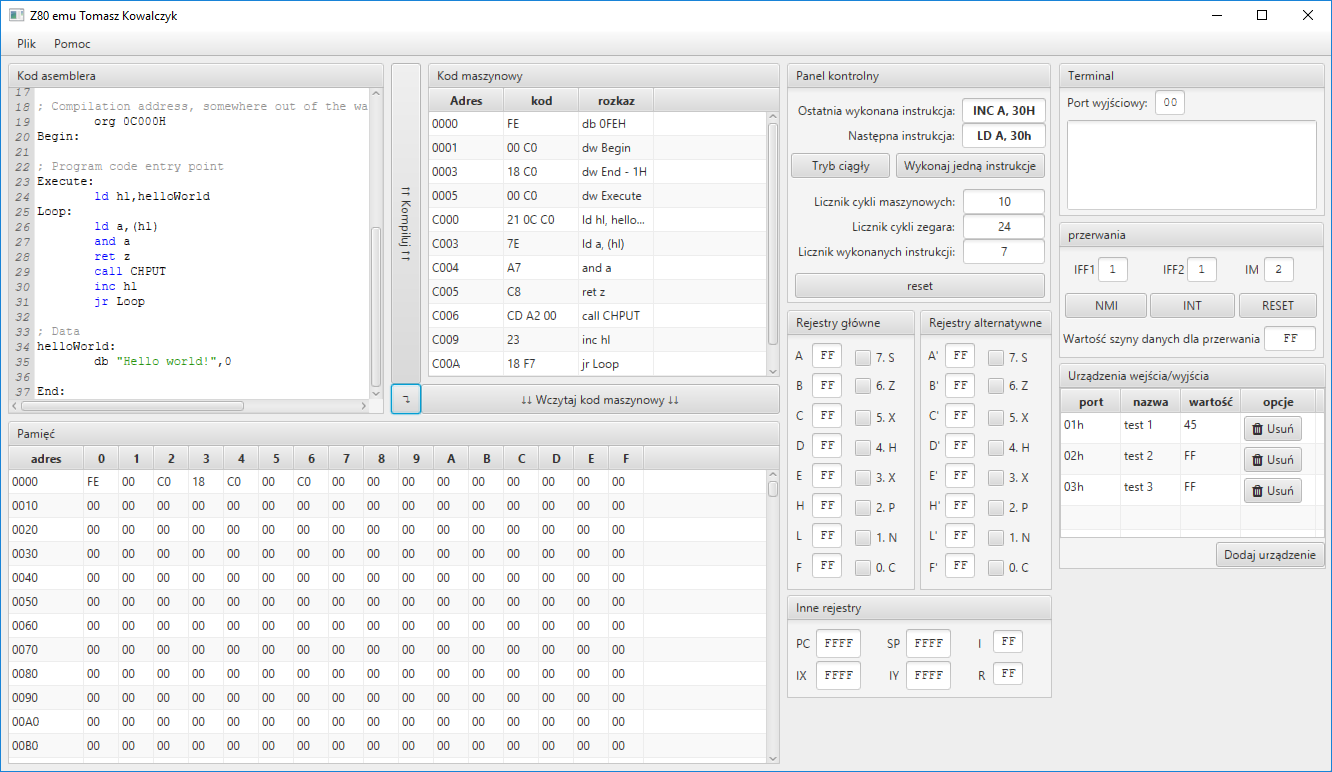
\includegraphics[width=1\textwidth]{z80Gui}
		\caption{Makieta interfejsu użytkownika}
		\label{img:z80Gui}
	\end{figure}
	 
	
	Elementy interfejsu użytkownika podzielono na dwa zbiory w celu czytelniejszego objaśnienia ich roli. Pierwszy zbiór zaprezentowany na grafice \ref{img:z80GuiPart1WithPoints} zawiera elementy związane ze sterowaniem pamięcią oraz kodem programu. Opis poszczególnych elementów umieszczonych na schemacie:
	\begin{enumerate}
		\item edytor kodu asemblera, z prostym kolorowaniem składni,
		\item widok kodu maszynowego w formie tabeli, zawierającej informacje o adresie rozkazu w pamięci, kodzie maszynowym oraz czytelnej dla człowieka nazwie instrukcji,
		\item tabela reprezentująca moduł pamięci podłączony do procesora,
		\item przycisk kompilujący kod asemblera (p. 1) do kodu maszynowego (p. 2),
		\item przycisk wczytujący kod maszynowy programu(p. 2), do pamięci procesora (p. 3),
		\item przycisk wykonujący kompilacje kodu asemblera (p. 1) a następnie wczytanie go do pamięci (p. 3).
	\end{enumerate}
	
	\begin{figure}[h]
		\centering
		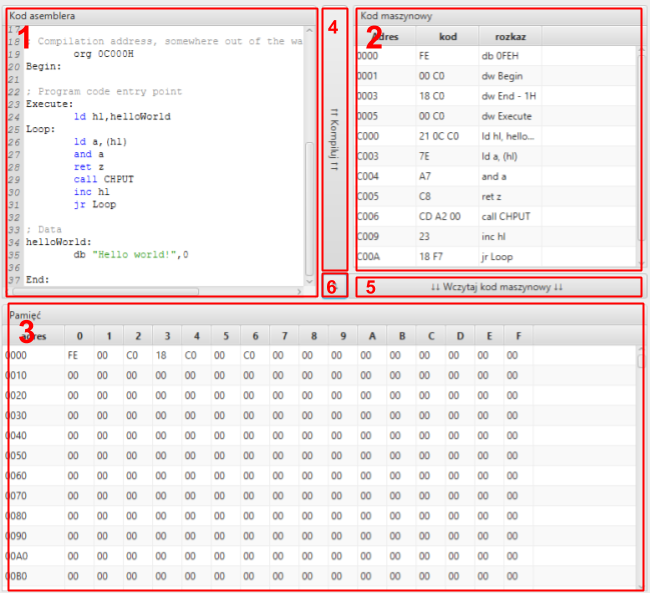
\includegraphics[width=1\textwidth]{z80GuiPart1WithPoints}
		\caption{Makieta interfejsu użytkownika z oznaczeniami. Część 1}
		\label{img:z80GuiPart1WithPoints}
	\end{figure}
	
	Drugą część interfejsu zaprezentowano na grafice \ref{img:z80GuiPart2WithPoints}. Oto opis poszczególnych elementów:
	\begin{enumerate}
		\item główny panel kontrolujący proces emulacji, przedstawiający między innymi liczbę cykli maszynowych i zegara wykonywanego programu,
		\item pola prezentujące nazwę ostatniej wykonanej i następnej w kolejce instrukcji procesora,
		\item przycisk uruchamiający emulację ciągłą (ponownie jego wybranie zatrzymuje emulacje),
		\item przycisk wykonujący pojedynczy, następny rozkaz procesora,
		\item przycisk resetujący urządzenie,
		\item widok rejestrów głównych i alternatywnych włącznie z flagami,
		\item widok rejestrów I, R, PC, SP, IX, IY,
		\item terminal wyjściowy, emulujący na stałe przypisane urządzenie,
		\item pole tekstowe, do którego wpisywany jest numer portu terminala wyjściowego, pod jakim będzie przyjmował on dane,
		\item panel grupujący elementy interfejsu odpowiedzialne za przerwania,
		\item przycisk generujący NMI (z ang. \emph{Non-Maskable Interrupt}), sygnał przerwania niemaskowanego,
		\item przycisk generujący INT (z ang. \emph{Interrupt}), sygnał maskowanego przerwania,
		\item przycisk generujący sygnał resetu,
		\item pole tekstowe zawierające 8{\dywiz}bitową wartość, jaką przyjmie szyna danych podczas zgłoszenia przerwania,
		\item tabela z listą podłączonych urządzeń wejścia/wyjścia,
		\item przycisk pozwalający na usunięcie urządzenia wejścia/wyjścia,
		\item przycisk dodający nowe urządzenie wejścia/wyjścia.
	\end{enumerate}
	
	\begin{figure}[h]
		\centering
		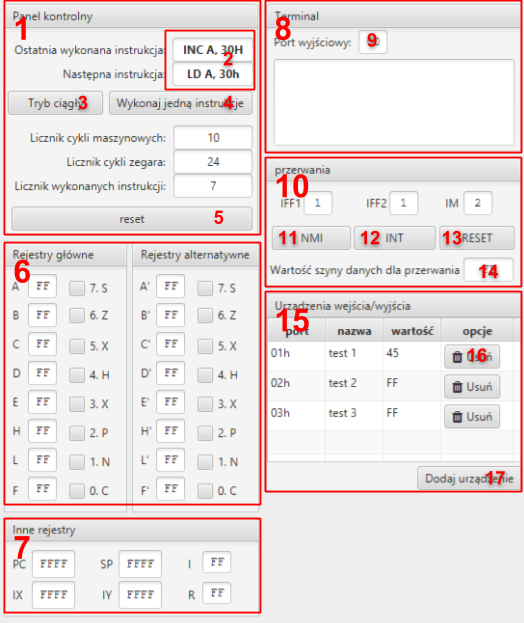
\includegraphics[width=0.8\textwidth]{z80GuiPart2WithPoints}
		\caption{Makieta interfejsu użytkownika z oznaczeniami. Część 2}
		\label{img:z80GuiPart2WithPoints}
	\end{figure}

	%tutaj o mvc
	
	W rozdziale opracowano wymagania funkcjonalne i niefunkcjonalne aplikacji. Zaprojektowano strukturę projektu podzieloną na trzy moduły. Głównym kryterium, jakie przyjęto podczas projektowania, jest możliwość ponownego użycia każdego z nich w innym projekcie emulatora. W ramach projektu stworzono także makietę interfejsu użytkownika w języku FXML.